% TikZ chains with labeled edges
% Author: Stefan Kottwitz , http://texblog.net
\documentclass{standalone}\usepackage[]{graphicx}\usepackage[]{color}
%% maxwidth is the original width if it is less than linewidth
%% otherwise use linewidth (to make sure the graphics do not exceed the margin)
\makeatletter
\def\maxwidth{ %
  \ifdim\Gin@nat@width>\linewidth
    \linewidth
  \else
    \Gin@nat@width
  \fi
}
\makeatother

\definecolor{fgcolor}{rgb}{0.345, 0.345, 0.345}
\newcommand{\hlnum}[1]{\textcolor[rgb]{0.686,0.059,0.569}{#1}}%
\newcommand{\hlstr}[1]{\textcolor[rgb]{0.192,0.494,0.8}{#1}}%
\newcommand{\hlcom}[1]{\textcolor[rgb]{0.678,0.584,0.686}{\textit{#1}}}%
\newcommand{\hlopt}[1]{\textcolor[rgb]{0,0,0}{#1}}%
\newcommand{\hlstd}[1]{\textcolor[rgb]{0.345,0.345,0.345}{#1}}%
\newcommand{\hlkwa}[1]{\textcolor[rgb]{0.161,0.373,0.58}{\textbf{#1}}}%
\newcommand{\hlkwb}[1]{\textcolor[rgb]{0.69,0.353,0.396}{#1}}%
\newcommand{\hlkwc}[1]{\textcolor[rgb]{0.333,0.667,0.333}{#1}}%
\newcommand{\hlkwd}[1]{\textcolor[rgb]{0.737,0.353,0.396}{\textbf{#1}}}%

\usepackage{framed}
\makeatletter
\newenvironment{kframe}{%
 \def\at@end@of@kframe{}%
 \ifinner\ifhmode%
  \def\at@end@of@kframe{\end{minipage}}%
  \begin{minipage}{\columnwidth}%
 \fi\fi%
 \def\FrameCommand##1{\hskip\@totalleftmargin \hskip-\fboxsep
 \colorbox{shadecolor}{##1}\hskip-\fboxsep
     % There is no \\@totalrightmargin, so:
     \hskip-\linewidth \hskip-\@totalleftmargin \hskip\columnwidth}%
 \MakeFramed {\advance\hsize-\width
   \@totalleftmargin\z@ \linewidth\hsize
   \@setminipage}}%
 {\par\unskip\endMakeFramed%
 \at@end@of@kframe}
\makeatother

\definecolor{shadecolor}{rgb}{.97, .97, .97}
\definecolor{messagecolor}{rgb}{0, 0, 0}
\definecolor{warningcolor}{rgb}{1, 0, 1}
\definecolor{errorcolor}{rgb}{1, 0, 0}
\newenvironment{knitrout}{}{} % an empty environment to be redefined in TeX

\usepackage{alltt}
\usepackage{tikz}
\usepackage{fontspec}
\usetikzlibrary{matrix,positioning,scopes}
% %
% \makeatletter
% \tikzset{join/.code=\tikzset{after node path={%
% \ifx\tikzchainprevious\pgfutil@empty\else(\tikzchainprevious)%
% edge[every join]#1(\tikzchaincurrent)\fi}}}
% \makeatother
% %
% \tikzset{>=stealth',every on chain/.append style={join},
%          every join/.style={->}}
% \tikzstyle{labeled}=[execute at begin node=$\scriptstyle,
%    execute at end node=$]
%
\IfFileExists{upquote.sty}{\usepackage{upquote}}{}
\begin{document}
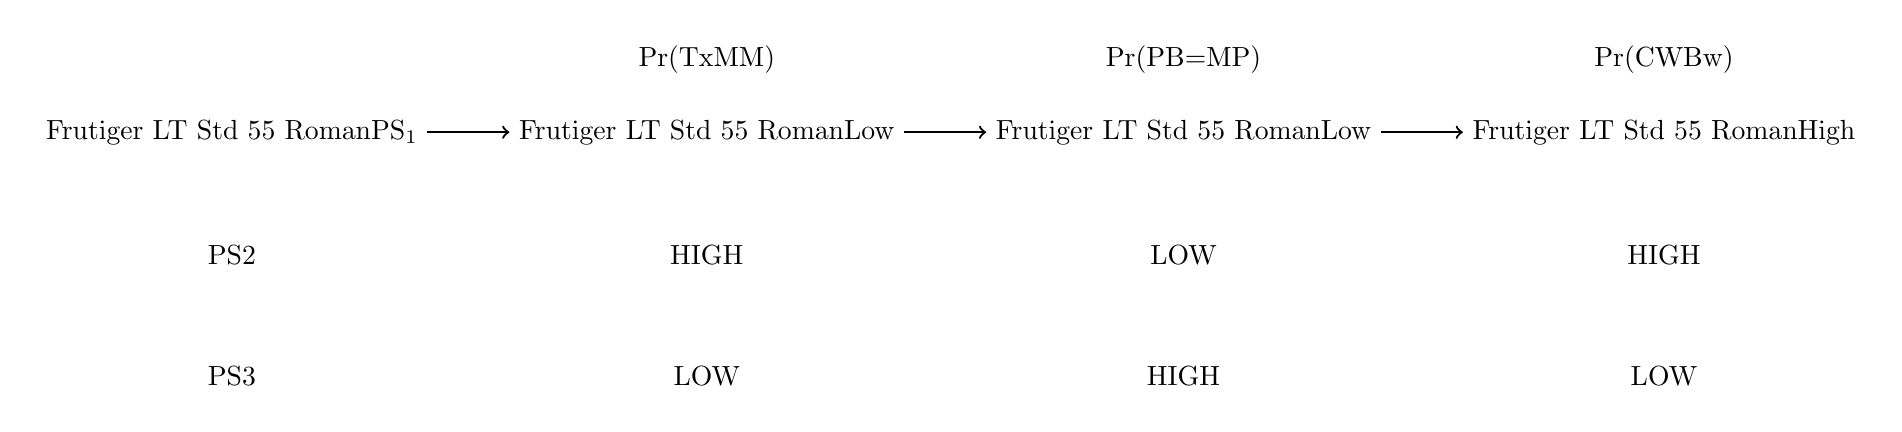
\begin{tikzpicture}
  \matrix (m) [matrix of nodes, row sep=3em, column sep=3em]
    { {} & Pr(TxMM)  & Pr(PB=MP)  & Pr(CWBw) \\ [-20pt]
    \fontspec{Frutiger LT Std 55 Roman}PS\textsubscript{1} & 
      \fontspec{Frutiger LT Std 55 Roman}Low  & 
      \fontspec{Frutiger LT Std 55 Roman}Low  & 
      \fontspec{Frutiger LT Std 55 Roman}High \\
      PS2 & HIGH & LOW & HIGH  \\
      PS3 & LOW  & HIGH & LOW  \\};
    
    %{ [start chain] 
     % \chainin (m-2-1);
      %\chainin (m-2-2);
      %\chainin (m-2-3);
      %\chainin (m-2-4);
    %}
%     { [start chain] 
%       \chainin (m-3-1);
%       \chainin (m-3-2);
%       \chainin (m-3-3);
%       \chainin (m-3-4);
%     }
%     { [start chain] 
%       \chainin (m-4-1);
%       \chainin (m-4-2);
%       \chainin (m-4-3);
%       \chainin (m-4-4);
%     }
    \path[thick,->] (m-2-1) edge (m-2-2);
    \path[thick,->] (m-2-2) edge (m-2-3);
    \path[thick,->] (m-2-3) edge (m-2-4);
\end{tikzpicture}
\end{document}
